\begin{figure}[t!]
\centering

\resizebox{1.0\linewidth}{!}{ %
\setlength{\tabcolsep}{8pt} % Adjust column spacing if needed
\renewcommand{\arraystretch}{1.2} % Adjust row spacing if needed
\begin{tabular}{>{\centering\arraybackslash}m{0.25\textwidth} 
                >{\centering\arraybackslash}m{0.25\textwidth} 
                >{\centering\arraybackslash}m{0.25\textwidth}}
    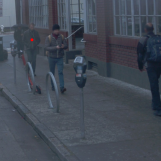
\includegraphics[width=0.27\textwidth]{Figures/lidar_hpc_subfigures/rgb_1557962430313036.png} &
    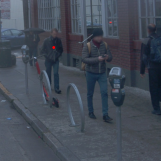
\includegraphics[width=0.27\textwidth]{Figures/lidar_hpc_subfigures/rgb_1557962431112927.png} &
    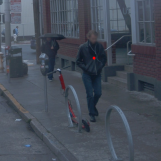
\includegraphics[width=0.27\textwidth]{Figures/lidar_hpc_subfigures/rgb_1557962431812796.png} \\


    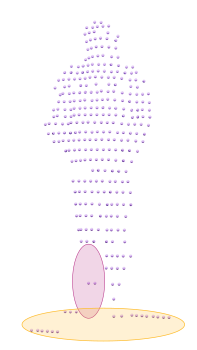
\includegraphics[width=0.22\textwidth]{Figures/lidar_hpc_subfigures/human1.png} &
    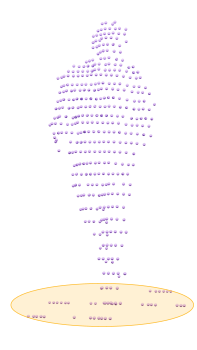
\includegraphics[width=0.22\textwidth]{Figures/lidar_hpc_subfigures/human2.png} &
    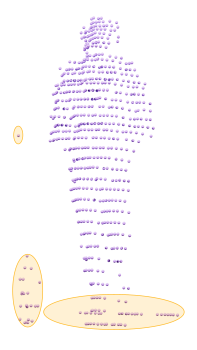
\includegraphics[width=0.22\textwidth]{Figures/lidar_hpc_subfigures/human3.png} \\
    \Large{314 pts @ 16.7 m} & \Large{416 pts @ 13.9 m} & \Large{617 pts @ 10.8 m} \\[2ex]
\end{tabular}
}
\caption{\textbf{LiDAR human point cloud challenges} include noise, occlusions, and significant variations in point cloud density. The top rows show raw images and their corresponding human point clouds extracted from Waymo Open Dataset~\cite{sunScalabilityPerceptionAutonomous2020}. The subject of interest is marked with a red dot on the chest. The bottom row indicates the distance to the sensor (in meters) and the corresponding number of LiDAR points (pts). \textcolor{mh4}{\textbf{Occlusion}} of the right shin in the first frame; \textcolor{mh7}{\textbf{persistent noise}} near the feet; and point density is observed to increase as the subject moves closer to the sensor.}
\label{fig:lidar_hpc_challenges}
\end{figure}